\begin{figure}[!htbp]
    \centering
    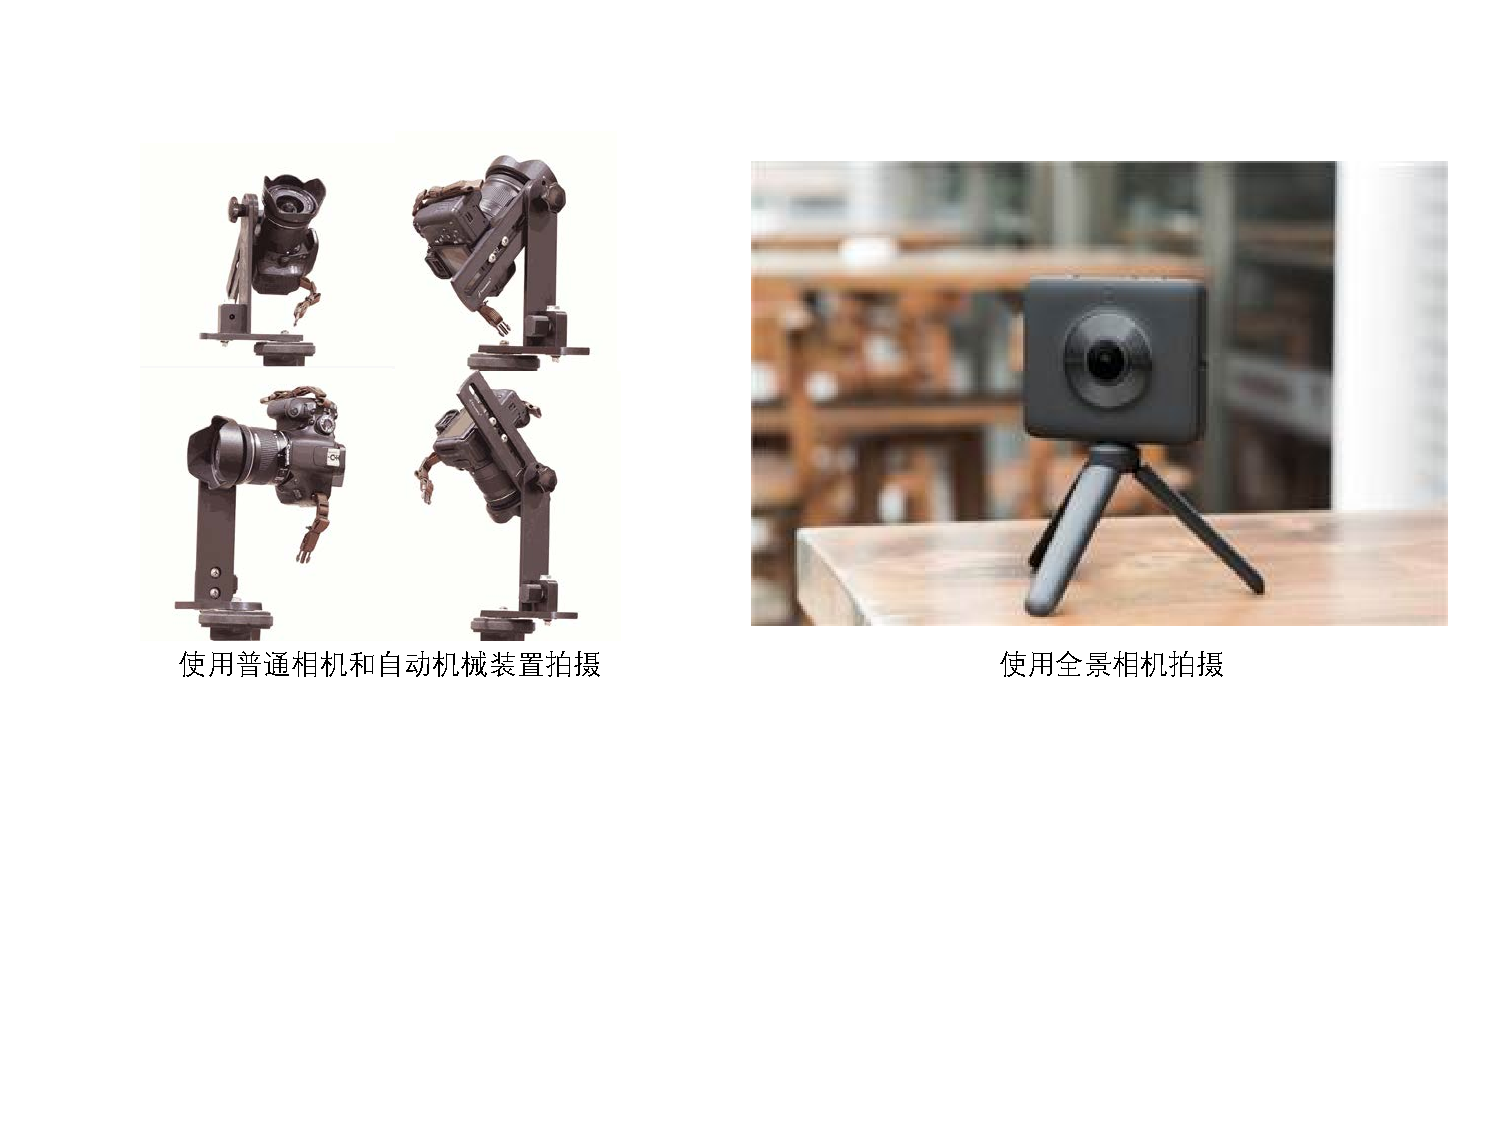
\includegraphics[width=1.0\textwidth]{Img/capture-panorama.pdf}
    \caption[拍摄全景图的示例]
    {常见的拍摄全景图的方式。左图是将单反相机固定在能够自动控制旋转的机械架上,对多个方向进行拍摄,最后利用电脑软件将其拼接到一起;右图是使用全景相机拍摄,由于鱼眼镜头和内置硬件的帮助,这种拍摄方式十分简便,只需一次拍摄就可以获得整个全景图。}
    \label{fig:capture-panorama}
\end{figure}